\section{Experiments}
\label{sec:experiments}

Step-independent training collapses while episode-level training succeeds; a partial factorial design separates the two mechanisms; and window size $h$ modulates severity.

\subsection{Setup}
\label{sec:setup}

We evaluate on ALFWorld~\citep{shridhar2021alfworld}, a text-based household environment with six task types requiring sequential reasoning over up to 50 steps. The environment provides ternary reward ($r_- {=} {-}0.1$ per invalid action, $0$ for valid but unsuccessful, $r_+$ for success); our theory assumes simplified binary reward ($R \in \{0, r_+\}$), yielding an upper bound on sign misattribution (Section~\ref{sec:sign_verification} validates under both). The base policy is Qwen3-1.7B~\citep{qwen3_2025} fine-tuned on expert demonstrations (SFT baseline: 12.5\% in-distribution), where Proposition~2 predicts the majority of gradient updates carry incorrect sign. All conditions use RAGEN~\citep{ragen2025} (v0.1)\footnote{Our implementation extends RAGEN v0.1 with episode-level training support. Code available upon acceptance.} with GRPO~\citep{shao2024deepseekmath} ($K{=}8$; Appendix~\ref{app:hyperparameters}). We report success rate on a 134-task OOD set (primary) and 32-task in-distribution set (secondary).

\subsection{Partial Factorial Mechanism Separation}
\label{sec:factorial_experiments}

We implement the partial factorial design from Section~\ref{sec:factorial_design} (3 of 4 cells; Cell~C excluded due to NaN instability; Appendix~\ref{app:cell_c}) with two seeds per condition. Cell~C's qualitatively different failure (divergence rather than gradual collapse) suggests information loss may unintentionally stabilize gradient variance, questioning exact separability (Section~\ref{sec:discussion}).

\subsection{Results}
\label{sec:results}

Cell~A collapses in two phases (Table~\ref{tab:main_results}): task success drops to ${\leq}$3\% by step~5 and remains below 10\% through step~15, while action validity initially remains high; continued sign misattribution then destroys even basic formatting.
Cell~B eliminates sign misattribution while retaining information loss: training success improves, but OOD generalization (5.97\%) remains near the SFT baseline (6.72\%), confirming that removing M2 alone bounds learning without causing degradation.
Cell~D is the only condition that substantially exceeds the SFT baseline, with monotonic OOD improvement across both seeds.
The A$\to$B comparison isolates M2; the B$\to$D comparison isolates M1. Both mechanisms are necessary to explain the full failure pattern (Figure~\ref{fig:hsweep}a).

\begin{table}[t]
\centering
\caption{1.7B results on ALFWorld (best checkpoint per seed). Full seed-level breakdown in Table~\ref{tab:seed_variability} and Appendix~\ref{tab:additional_baselines}.}
\label{tab:main_results}
\resizebox{\columnwidth}{!}{%
\begin{tabular}{@{}llccc@{}}
\toprule
\textbf{Condition} & \textbf{Mechanisms} & \textbf{Best Step} & \textbf{In-Dist (\%)} & \textbf{OOD (\%)} \\
\midrule
SFT baseline & --- & --- & 12.50 & 6.72 \\
Cell A ($h{=}2$, step) & M1+M2 & 5 & 1.56$^\S$ & --- \\
Cell B ($h{=}2$, episode) & M1 only & 5 & 18.75 & 5.97$^\ast$ \\
Cell D (full, episode) & neither & 15 & \textbf{34.38} & \textbf{17.16} \\
\bottomrule
\end{tabular}}
\begin{flushleft}
\small $^\ast$ Single seed; seed2 best checkpoint unavailable for re-evaluation. \\
\small $^\S$ Mean of two seeds (0\% and 3.13\%); seed~1 collapses to 0\% by step~15; seed~2 shows partial recovery (9.4\%). OOD not evaluated at this checkpoint.
\end{flushleft}
\end{table}

\paragraph{Additional conditions.} Dense reward, REINFORCE++, and discount-factor sweep experiments suggest that sign misattribution, not reward sparsity or discounting, drives the failure (Appendix~\ref{app:additional}).

\paragraph{Window-size sweep.} Varying window size reveals $h{=}10$ as a seed-dependent boundary (Figure~\ref{fig:hsweep}b). Windows of $h{\leq}5$ collapse to 0\% across all seeds; $h{=}20$ and full-episode conditions recover monotonically. At $h{=}10$, two seeds diverge (6.25\% vs.\ 21.9\%, mean 14.1\%), placing this window size at the instability boundary rather than in a deterministic collapse zone. All other conditions are single-seed.
\label{sec:results_hsweep}

\subsection{Sign Misattribution Verification}
\label{sec:sign_verification}

We distinguish three metrics that each capture a different aspect of credit assignment quality:

\textit{(1) Sign-episode correlation}: whether advantage sign tracks episode outcome. Under binary reward (penalty${=}0$), correlation is near-perfect at 99.6\% ($270/271$ non-zero windows; Figure~\ref{fig:sign_misattribution}), directly confirming M2: advantage sign is determined by episode outcome, not local action quality.\footnote{The single discordant window arises from GRPO group-composition effects, not a violation of the mechanism.} This follows by construction, since all windows in a successful episode share the same positive return.

\textit{(2) Credit agreement rate}: whether advantage sign matches local action quality, operationalized via action validity as a proxy (Definition~1). Under penalty reward ($h{=}2$, $n{=}3{,}000$ windows), only 52.07\% of valid-action windows receive positive advantage ($p{=}0.025$ vs.\ 50\%; Cohen's $h \approx 0.041$, below the small-effect threshold), confirming near-random credit agreement. Under binary reward, agreement drops to 28\% ($n{=}271$), as advantage sign systematically penalizes valid actions in failed episodes. This metric is an upper bound: valid actions include strategically suboptimal moves, yet agreement remains near-random even under this generous criterion.

\textit{(3) $P(\text{correct} \mid \text{update})$}: the theoretical upper bound from Proposition~2 ($\leq$19.1\% at $p{=}12.5\%$, $K{=}8$). This bounds the fraction of non-zero gradient updates with correct sign, a different quantity from the credit agreement rate, which conditions on action validity rather than gradient participation. The two metrics are complementary: Proposition~2 bounds worst-case gradient quality; credit agreement measures empirical signal strength.

The empirical magnitude ratio $|\hat{A}_{\text{correct}}|/|\hat{A}_{\text{wrong}}| \approx 2.6$ at step~5 ($n{=}30$) falls below the break-even threshold $(1{-}P_c)/P_c \approx 4.2$, confirming magnitude asymmetry cannot compensate for sign frequency (Section~\ref{sec:theory}). Combined with $\gamma{=}1.0$ collapse (Appendix~\ref{app:additional}), these measurements support sign misattribution as a primary factor, though the credit agreement effect is small ($+$2pp).

\begin{figure}[t]
\centering
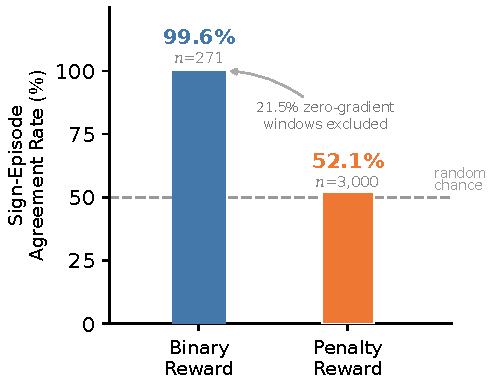
\includegraphics[width=\columnwidth]{fig_sign_misattribution.pdf}
\caption{Sign-episode correlation (binary reward) vs.\ credit agreement rate (penalty reward). Under binary reward, advantage sign tracks episode outcome near-perfectly, confirming M2. Under penalty reward, credit agreement drops to near-random chance (dashed line).}
\label{fig:sign_misattribution}
\end{figure}

\subsection{Episode-Level Training: Seed Variability}
\label{sec:seed_variability}

Episode-level GRPO addresses the dual-mechanism failure, but outcomes remain seed-dependent. We evaluate $N{=}11$ seeds under identical hyperparameters, classifying each as \textbf{collapsed} (in-distribution success declines $>$50\% from peak for $\geq$3 steps), \textbf{stagnant} (stable but not significant vs.\ SFT), or \textbf{generalized} (Fisher exact $p{<}0.01$ vs.\ SFT on the 134-task OOD set). Table~\ref{tab:seed_variability} reports best-checkpoint results per seed.

\begin{table}[t]
\centering
\caption{Episode-level GRPO across 11 seeds (134 OOD tasks, best checkpoint per seed). C=Collapsed, S=Stagnant, G=Generalized (Fisher exact $p{<}0.01$ vs.\ SFT). NS=not significant. Wilson 95\% confidence interval. SFT baseline: 6.72\%.}
\label{tab:seed_variability}
\resizebox{\columnwidth}{!}{%
\begin{tabular}{@{}llcccc@{}}
\toprule
\textbf{Seed} & \textbf{Step} & \textbf{Cat.} & \textbf{OOD (\%)} & \textbf{95\% CI} & \textbf{vs SFT} \\
\midrule
seed2048$^\ddagger$ & 5 & C & 8.21 & [4.6, 14.2] & NS \\
seed42$^\ddagger$ & 5 & C & 12.69 & [8.0, 19.4] & NS \\
seed8 & 5 & C & 11.94 & [7.5, 18.5] & NS \\
\midrule
seed200 & 5 & S & 10.45 & [6.3, 16.8] & NS \\
seed300 & 5 & S & 10.45 & [6.3, 16.8] & NS \\
seed100 & 10 & S & 12.69 & [8.0, 19.4] & NS \\
seed2$^\ddagger$ & 15 & S & 15.67 & [10.5, 22.8] & $p{=}0.03$ \\
\midrule
seed1 & 5 & G$^\dagger$ & 23.88 & [17.4, 31.8] & $p{<}0.001$ \\
seed5 & 10 & G & 29.10 & [22.1, 37.3] & $p{<}0.001$ \\
seed6 & 15 & G & 29.10 & [22.1, 37.3] & $p{<}0.001$ \\
seed4 & 15 & G & 30.60 & [23.5, 38.7] & $p{<}0.001$ \\
\bottomrule
\end{tabular}}
\begin{flushleft}
\small $^\dagger$ RAGEN built-in eval; checkpoint unavailable for re-evaluation. \\
\small $^\ddagger$ OOD evaluated via RAGEN built-in eval; not independently re-evaluated under 134-task OOD evaluation protocol. \\
\small All results are single-run evaluations at decoding temperature $\tau{=}0.4$; see Limitations for eval variance discussion.
\end{flushleft}
\end{table}

\begin{figure}[t]
\centering\vspace{-3pt}
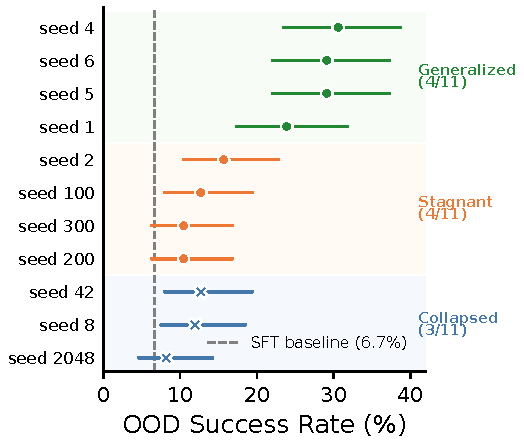
\includegraphics[width=0.95\columnwidth]{fig_seed_variability.pdf}\vspace{-5pt}
\caption{OOD success rate across 11 episode-level GRPO seeds (Wilson 95\% CI). Seeds partition into \textit{Generalized} ($p{<}0.01$ vs.\ SFT), \textit{Stagnant} (stable, NS), and \textit{Collapsed} ($\times$). Avoiding collapse is necessary but not sufficient.}
\label{fig:seed_variability}\vspace{-8pt}
\end{figure}

Three outcomes emerge (Table~\ref{tab:seed_variability}, Figure~\ref{fig:seed_variability}): ${\sim}$27\% collapse with response length inflation (Appendix~\ref{app:response_length}), ${\sim}$36\% stagnate near SFT, and ${\sim}$36\% generalize. The 11-seed mean OOD success rate is 17.7\%, compared to the SFT baseline of 6.72\%. Unified step-5 evaluation across all seeds guards against checkpoint selection bias (Appendix~\ref{app:step5_unified}). Stable training is necessary but not sufficient; the mechanism driving seed-dependent transfer remains open (Section~\ref{sec:discussion}).

\subsection{Cross-Scale and Cross-Environment Verification}
\label{sec:cross_scale}

A single-seed 8B experiment confirms both failure and fix persist at scale: Cell~A collapses within two steps while Cell~D reaches 90.3\% OOD (Appendix~\ref{app:8b_results}); restricting to $h{=}2$ confirms severe information loss. The pathology is environment-general: step-independent training on ScienceWorld~\citep{wang2022scienceworld} also collapses to 0\% across all 15 steps with comparable M1 gap.
